\chapter{Proposed Method}
\label{chap:method}

This chapter presents the two proposed frameworks. Section~\ref{sec:backflush_method} introduces BackFlush, a knowledge-free framework for backdoor detection and elimination with watermark preservation. Section~\ref{sec:repair_method} introduces RePAIR, a framework for interactive machine unlearning through prompt-aware model repair. Both frameworks are grounded in machine unlearning but operate under fundamentally different constraints and address distinct threat models as formalized in Chapter~\ref{chap:threat_model}.


%% ============================================================
\section{BackFlush: Backdoor Detection and Elimination with Watermark Preservation}\label{sec:backflush_method}
%% ============================================================

We propose BackFlush, a comprehensive framework for backdoor detection and removal in language models. The framework requires no prior knowledge of trigger patterns, payload content, or poisoning methodology.

%% ------------------------------------------------------------
\subsection{Overview}\label{subsec:bf_overview}
%% ------------------------------------------------------------

Given a suspect model $\mathcal{M}_s$, the framework operates in three stages, namely detection via Backdoor Susceptibility Amplification, auxiliary data injection, and Rotation-based Parameter Editing (RoPE) unlearning. Let $\mathcal{D}_{\textit{benign}}$ denote the benign training data and $\mathcal{D}_{\textit{aux}}$ denote auxiliary clean data. The complete pipeline is:

\begin{equation}
\mathcal{M}' = 
\begin{cases}
\mathcal{G}(\mathcal{M}_s, \mathcal{D}_{\textit{benign}}, \mathcal{D}_{\textit{aux}}) & \text{if } \mathcal{F}(\mathcal{M}_s, \mathcal{M}_{\textit{clean}}, \mathcal{D}_{\textit{probe}}) = 1 \\
\mathcal{M}_s & \text{otherwise}
\end{cases}
\end{equation}

If the detection function $\mathcal{F}$ identifies $\mathcal{M}_s$ as backdoored, the defense function $\mathcal{G}$ is applied, otherwise the model is returned unchanged.

%% ------------------------------------------------------------
\subsection{Backdoor Detection via Backdoor Susceptibility Amplification}\label{subsec:bf_detection}
%% ------------------------------------------------------------

Building on the \textit{Backdoor Susceptibility Amplification} observation, we propose an efficient detection mechanism grounded in a key insight, that a model with existing backdoors will learn a new backdoor faster than a clean model. Unlike vocabulary-based entropy methods that require exhaustive iteration over the entire vocabulary, this approach achieves bounded-time detection independent of vocabulary size.

Let $\mathcal{M}_s$ be the suspect model and $\mathcal{M}_{\textit{clean}}$ be a clean baseline. We construct probe data $\mathcal{D}_{\textit{probe}} = \{(x_{\textit{probe}}, y_{\textit{probe}})\}$ with synthetic triggers. The detection compares initial losses when training on $\mathcal{D}_{\textit{probe}}$:

\begin{equation}
\begin{aligned}
\mathcal{L}_{\textit{probe}}^{(s)} &= \mathbb{E}_{(x,y) \sim \mathcal{D}_{\textit{probe}}} \left[ \ell\left(\mathcal{M}_{\theta_s}(x), y\right) \right] \\
\mathcal{L}_{\textit{probe}}^{(\text{clean})} &= \mathbb{E}_{(x,y) \sim \mathcal{D}_{\textit{probe}}} \left[ \ell\left(\mathcal{M}_{\theta_{\textit{clean}}}(x), y\right) \right]
\end{aligned}
\end{equation}

where $\mathcal{L}_{\textit{probe}}^{(s)}$ and $\mathcal{L}_{\textit{probe}}^{(\text{clean})}$ denote the probe losses of the suspect model with parameters $\theta_s$ and the clean baseline with parameters $\theta_{\textit{clean}}$ respectively. The detection function returns:

\begin{equation}
\mathcal{F}(\mathcal{M}_s, \mathcal{M}_{\textit{clean}}, \mathcal{D}_{\textit{probe}}) = \mathbb{I}\left[ \mathcal{L}_{\textit{probe}}^{(\text{clean})} - \mathcal{L}_{\textit{probe}}^{(s)} > \tau \right]
\end{equation}

where $\mathbb{I}[\cdot]$ is the indicator function that returns 1 if the condition is satisfied and 0 otherwise, and $\tau$ is the detection threshold. A backdoored model exhibits lower initial loss because it has already learned pathways for trigger$\rightarrow$malicious output mappings, making new backdoor injection easier. This parallels Membership Inference Attacks, where adversaries classify samples by analyzing loss distributions. Here, we classify \textit{models} as backdoored or clean using the same principle.

%% ------------------------------------------------------------
\subsection{Phase 1: Auxiliary Data Injection}\label{subsec:bf_phase1}
%% ------------------------------------------------------------

If $\mathcal{F}(\mathcal{M}_s, \mathcal{M}_{\textit{clean}}, \mathcal{D}_{\textit{probe}}) = 1$, we proceed with backdoor removal. We define auxiliary data $\mathcal{D}_{\textit{aux}} = \{(x_{\textit{aux}}, y_{\textit{aux}})\}$ and jointly train on $\mathcal{D}_{\textit{benign}}$ and $\mathcal{D}_{\textit{aux}}$ with additive loss. Initially, the suspect model does not satisfy the auxiliary mapping:

\begin{equation}
\mathcal{M}_s : \mathcal{X}_{\textit{aux}} \cancel{\rightarrow} \mathcal{Y}_{\textit{aux}}
\end{equation}

where $\mathcal{X}_{\textit{aux}}$ and $\mathcal{Y}_{\textit{aux}}$ denote the input and output spaces of the auxiliary data respectively, and $\cancel{\rightarrow}$ denotes a mapping that does not hold. The Phase~1 loss combines retain and auxiliary objectives:

\begin{equation}
\mathcal{L}_{\textit{phase1}} = \underbrace{\mathbb{E}_{\mathcal{D}_{\textit{benign}}}\left[\ell(\mathcal{M}_\theta(x_{\textit{benign}}), y_{\textit{benign}})\right]}_{\textit{retain loss}} + \underbrace{\mathbb{E}_{\mathcal{D}_{\textit{aux}}}\left[\ell(\mathcal{M}_\theta(x_{\textit{aux}}), y_{\textit{aux}})\right]}_{\textit{auxiliary loss}}
\end{equation}

This produces an intermediate model $\mathcal{M}_{\theta^*}$ that satisfies the auxiliary mapping $\mathcal{M}_{\theta^*} : \mathcal{X}_{\textit{aux}} \rightarrow \mathcal{Y}_{\textit{aux}}$, which was not satisfied by the original suspect model $\mathcal{M}_s$. The key mechanism underlying the subsequent backdoor removal is that this injection entangles auxiliary and backdoor representations in shared parameter subspaces, setting the stage for Phase~2 to disrupt these entangled associations.

%% ------------------------------------------------------------
\subsection{Phase 2: Unlearning Auxiliary Data via RoPE}\label{subsec:bf_phase2}
%% ------------------------------------------------------------

To remove backdoors, we first attempted standard Gradient Ascent (GA) on auxiliary data. The GA loss maximizes prediction error on $\mathcal{D}_{\textit{aux}}$:

\begin{equation}
\mathcal{L}_{\textit{GA}} = \underbrace{\mathbb{E}_{\mathcal{D}_{\textit{benign}}}\left[\ell(\mathcal{M}_\theta(x_{\textit{benign}}), y_{\textit{benign}})\right]}_{\textit{retain loss}} - \underbrace{\mathbb{E}_{\mathcal{D}_{\textit{aux}}}\left[\ell(\mathcal{M}_\theta(x_{\textit{aux}}), y_{\textit{aux}})\right]}_{\textit{unlearning loss}}
\end{equation}

While GA successfully removed backdoors, it corrupted the watermark signature $\mathcal{S}(\mathcal{M}_{\theta'}, k) = 0$, violating the watermark preservation objective defined in Chapter~\ref{chap:threat_model}. The strong unlearning signal from GA causes indiscriminate parameter degradation that disrupts both backdoor and watermark subspaces.

To preserve watermarks while unlearning, we employ Rotation-based Parameter Editing (RoPE), a subtle unlearning approach via embedding rotation. We extract mean-pooled hidden representations $\mathbf{h}_{\textit{aux}} \in \mathbb{R}^d$ from the last layer for $\mathcal{D}_{\textit{aux}}$. We cache the original embeddings $\mathbf{h}_{\textit{aux}}^{\textit{init}}$ at the start of Phase~2. The target direction is the opposite:

\begin{equation}
\mathbf{h}_{\textit{aux}}^{\perp} = -\mathbf{h}_{\textit{aux}}^{\textit{init}}
\end{equation}

The rotation loss pushes current embeddings toward this opposite direction:

\begin{equation}
\mathcal{L}_{\textit{rotate}} = 1 - \cos(\mathbf{h}_{\textit{aux}}, \mathbf{h}_{\textit{aux}}^{\perp})
\end{equation}

The total Phase~2 loss combines retain and rotation objectives:

\begin{equation}
\mathcal{L}_{\textit{phase2}} = \underbrace{\mathbb{E}_{\mathcal{D}_{\textit{benign}}}\left[\ell(\mathcal{M}_\theta(x_{\textit{benign}}), y_{\textit{benign}})\right]}_{\textit{retain loss}} + \underbrace{\mathcal{L}_{\textit{rotate}}}_{\textit{unlearning loss}}
\end{equation}

This rotational shift provides subtle unlearning that flushes out backdoors alongside $\mathcal{D}_{\textit{aux}}$ while preserving watermark integrity, yielding a recovered model $\mathcal{M}_{\theta'}$ with $\mathcal{S}(\mathcal{M}_{\theta'}, k) = 1$.

%% ------------------------------------------------------------
\subsection{Watermark Preservation}\label{subsec:bf_watermark}
%% ------------------------------------------------------------

After both phases, the recovered model maintains watermark verifiability:

\begin{equation}
\mathcal{S}(\mathcal{M}_{\theta'}, k) = \mathcal{S}(\mathcal{M}_\theta, k) = 1
\end{equation}

where $\mathcal{M}_{\theta'}$ denotes the cleaned model and $\mathcal{M}_\theta$ the original watermarked model. The rotation loss, bounded in $[0, 2]$, provides controlled updates targeting auxiliary subspaces while preserving watermark parameters. In contrast, GA's unbounded gradients cause indiscriminate degradation across all parameter subspaces, including those encoding the watermark. This distinction between bounded rotation and unbounded gradient ascent is the key mechanism enabling simultaneous backdoor elimination and watermark preservation.

\begin{figure}[!htbp]
    \centering
    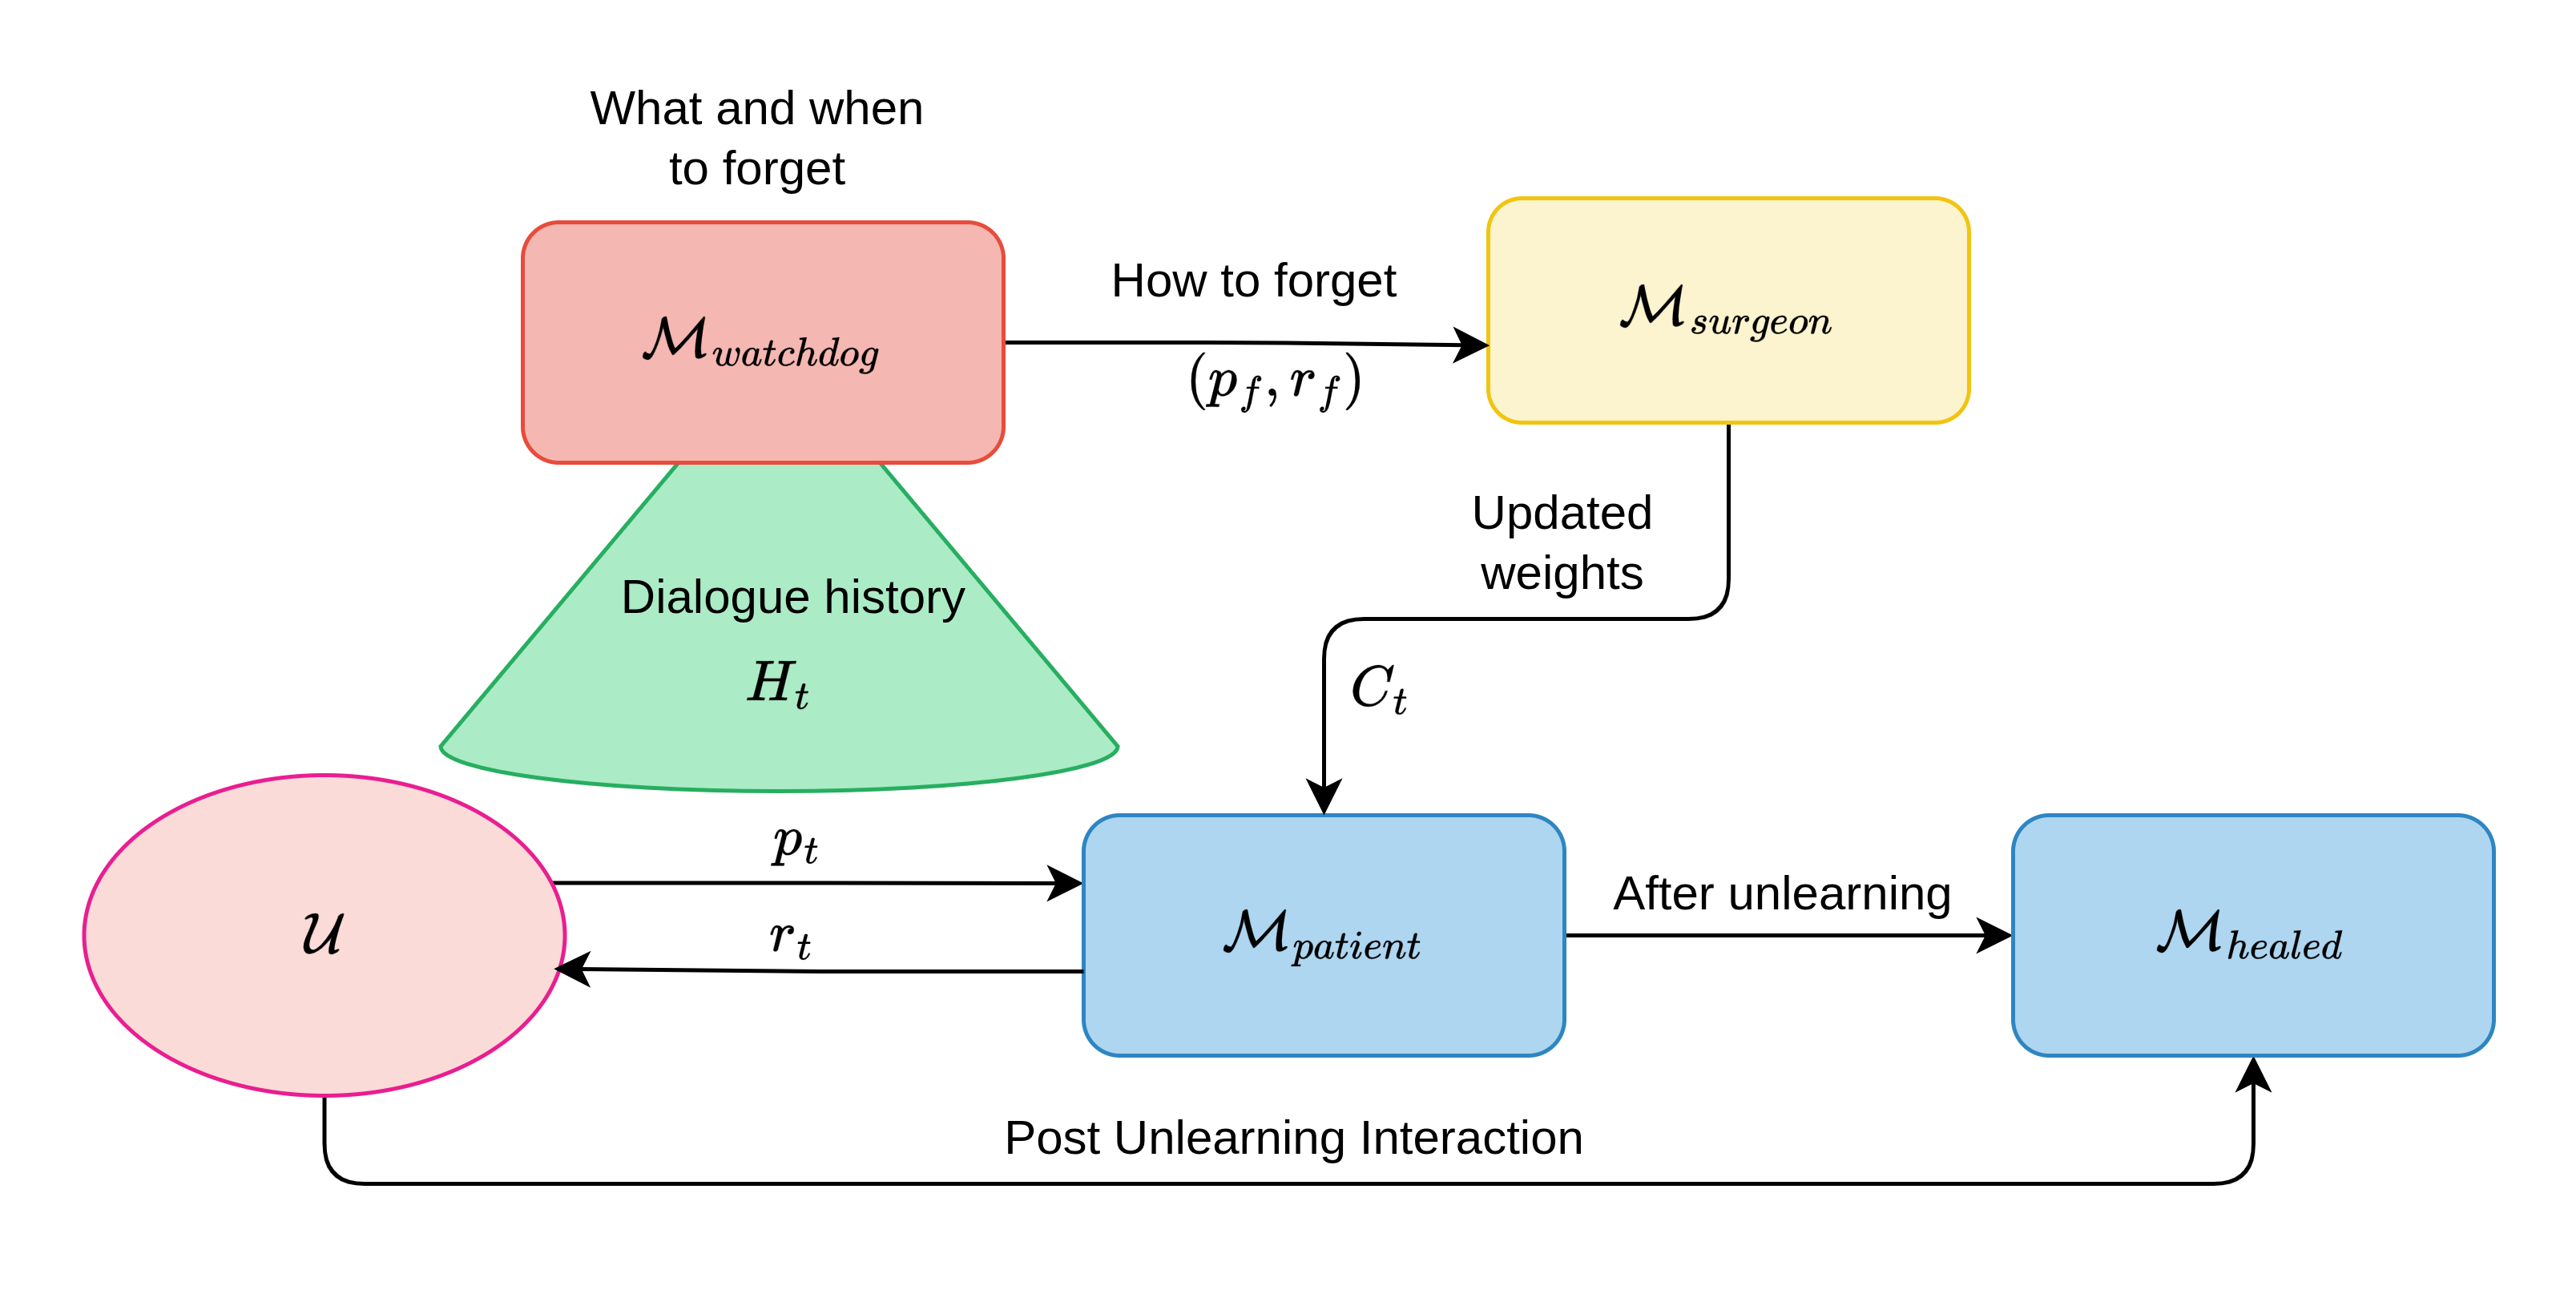
\includegraphics[width=0.5\linewidth]{Images/RePAIR/methodogy.png}
    \caption{Overview of the RePAIR framework: $\mathcal{M}_{\textit{watchdog}}$ detects unlearning requests and $\mathcal{M}_{\textit{surgeon}}$ repairs $\mathcal{M}_{\textit{patient}}$ into $\mathcal{M}_{\textit{healed}}$.}
    \label{fig:framework}
\end{figure}

%% ============================================================
\section{RePAIR: Interactive Machine Unlearning (IMU)}\label{sec:repair_method}
%% ============================================================

We propose \textbf{RePAIR} (Interactive Machine Unlearning through Prompt-Aware Model Repair), a framework for interactive machine unlearning with three components. The model $\mathcal{M}_{\textit{patient}}$ interacts with user $\mathcal{U}$ through prompts and responses, $\mathcal{M}_{\textit{watchdog}}$ monitors dialogue to detect \textit{what} and \textit{when} to forget, and $\mathcal{M}_{\textit{surgeon}}$ determines \textit{how} to forget by generating repair code that transforms $\mathcal{M}_{\textit{patient}}$ into $\mathcal{M}_{\textit{healed}}$.

%% ------------------------------------------------------------
\subsection{General Framework}\label{subsec:rp_framework}
%% ------------------------------------------------------------

Figure~\ref{fig:framework} illustrates the end-to-end RePAIR pipeline. During normal operation, $\mathcal{M}_{\textit{patient}}$ processes user prompts to produce responses $r_t = \mathcal{M}_{\textit{patient}}(p_t)$. In parallel, $\mathcal{M}_{\textit{watchdog}}$ monitors the dialogue history $H_t = \{(p_{t-k}, r_{t-k}), \ldots, (p_t, r_t)\}$ over the last $k$ turns and classifies the user's latest message as either \textit{chat} or \textit{unlearn}. Upon detecting an unlearn request, $\mathcal{M}_{\textit{watchdog}}$ extracts the target pair $(p_f, r_f)$ from $H_t$ and forwards it to $\mathcal{M}_{\textit{surgeon}}$, which generates the repair code $C_t = \mathcal{M}_{\textit{surgeon}}(p_f, r_f)$. The generated code invokes the STAMP unlearning procedure described in Section~\ref{subsec:rp_stamp}, which is training-free and operates on a single forget sample $(p_f, r_f)$, transforming $\mathcal{M}_{\textit{patient}}$ into $\mathcal{M}_{\textit{healed}}$. Post-unlearning, $\mathcal{U}$ interacts directly with $\mathcal{M}_{\textit{healed}}$.

%% ------------------------------------------------------------
\subsection{STAMP: Steering Through Activation Manipulation with Pseudoinverse}\label{subsec:rp_stamp}
%% ------------------------------------------------------------

We now describe the unlearning method that $\mathcal{M}_{\textit{surgeon}}$ executes on $\mathcal{M}_{\textit{patient}}$. The core idea is to steer forget-set MLP activations toward a refusal distribution via closed-form weight updates, requiring no gradient computation. As illustrated in Figure~\ref{fig:mlp_architecture}, each MLP layer in the SwiGLU architecture applies three weight matrices:

\begin{equation}
\mathbf{h} = \sigma(W_{\text{gate}} \cdot x) \odot (W_{\text{up}} \cdot x) \in \mathbb{R}^m, \qquad o = W_{\text{down}} \cdot \mathbf{h} \in \mathbb{R}^d
\end{equation}

where $x \in \mathbb{R}^d$ is the layer input, $\mathbf{h}$ is the post-activation intermediate, $\sigma$ is the SiLU activation function, and $\odot$ denotes element-wise multiplication. Throughout, $d$ denotes the residual-stream width and $m$ the larger FFN intermediate width, so that $W_{\text{gate}}, W_{\text{up}} \in \mathbb{R}^{m \times d}$ and $W_{\text{down}} \in \mathbb{R}^{d \times m}$. For Llama-3-8B, $d = 4096$ and $m = 14336$. Distinguishing $d$ from $m$ is essential, because the pseudoinverse solve below operates in $\mathbb{R}^m$ rather than $\mathbb{R}^d$.

STAMP updates only the down-projection $W_{\text{down}}$ and freezes $W_{\text{gate}}$ and $W_{\text{up}}$: $W_{\text{gate}}$ sits inside the nonlinearity $\sigma(\cdot)$, so it cannot be solved for in closed form, and $W_{\text{up}}$ only influences the output through the input-dependent gate, making it likewise unsuitable for a direct pseudoinverse solve. $W_{\text{down}}$, by contrast, maps linearly from $\mathbf{h}$ onto the MLP output, which is exactly the closed-form pseudoinverse update STAMP requires.

\begin{figure}[!htbp]
    \centering
    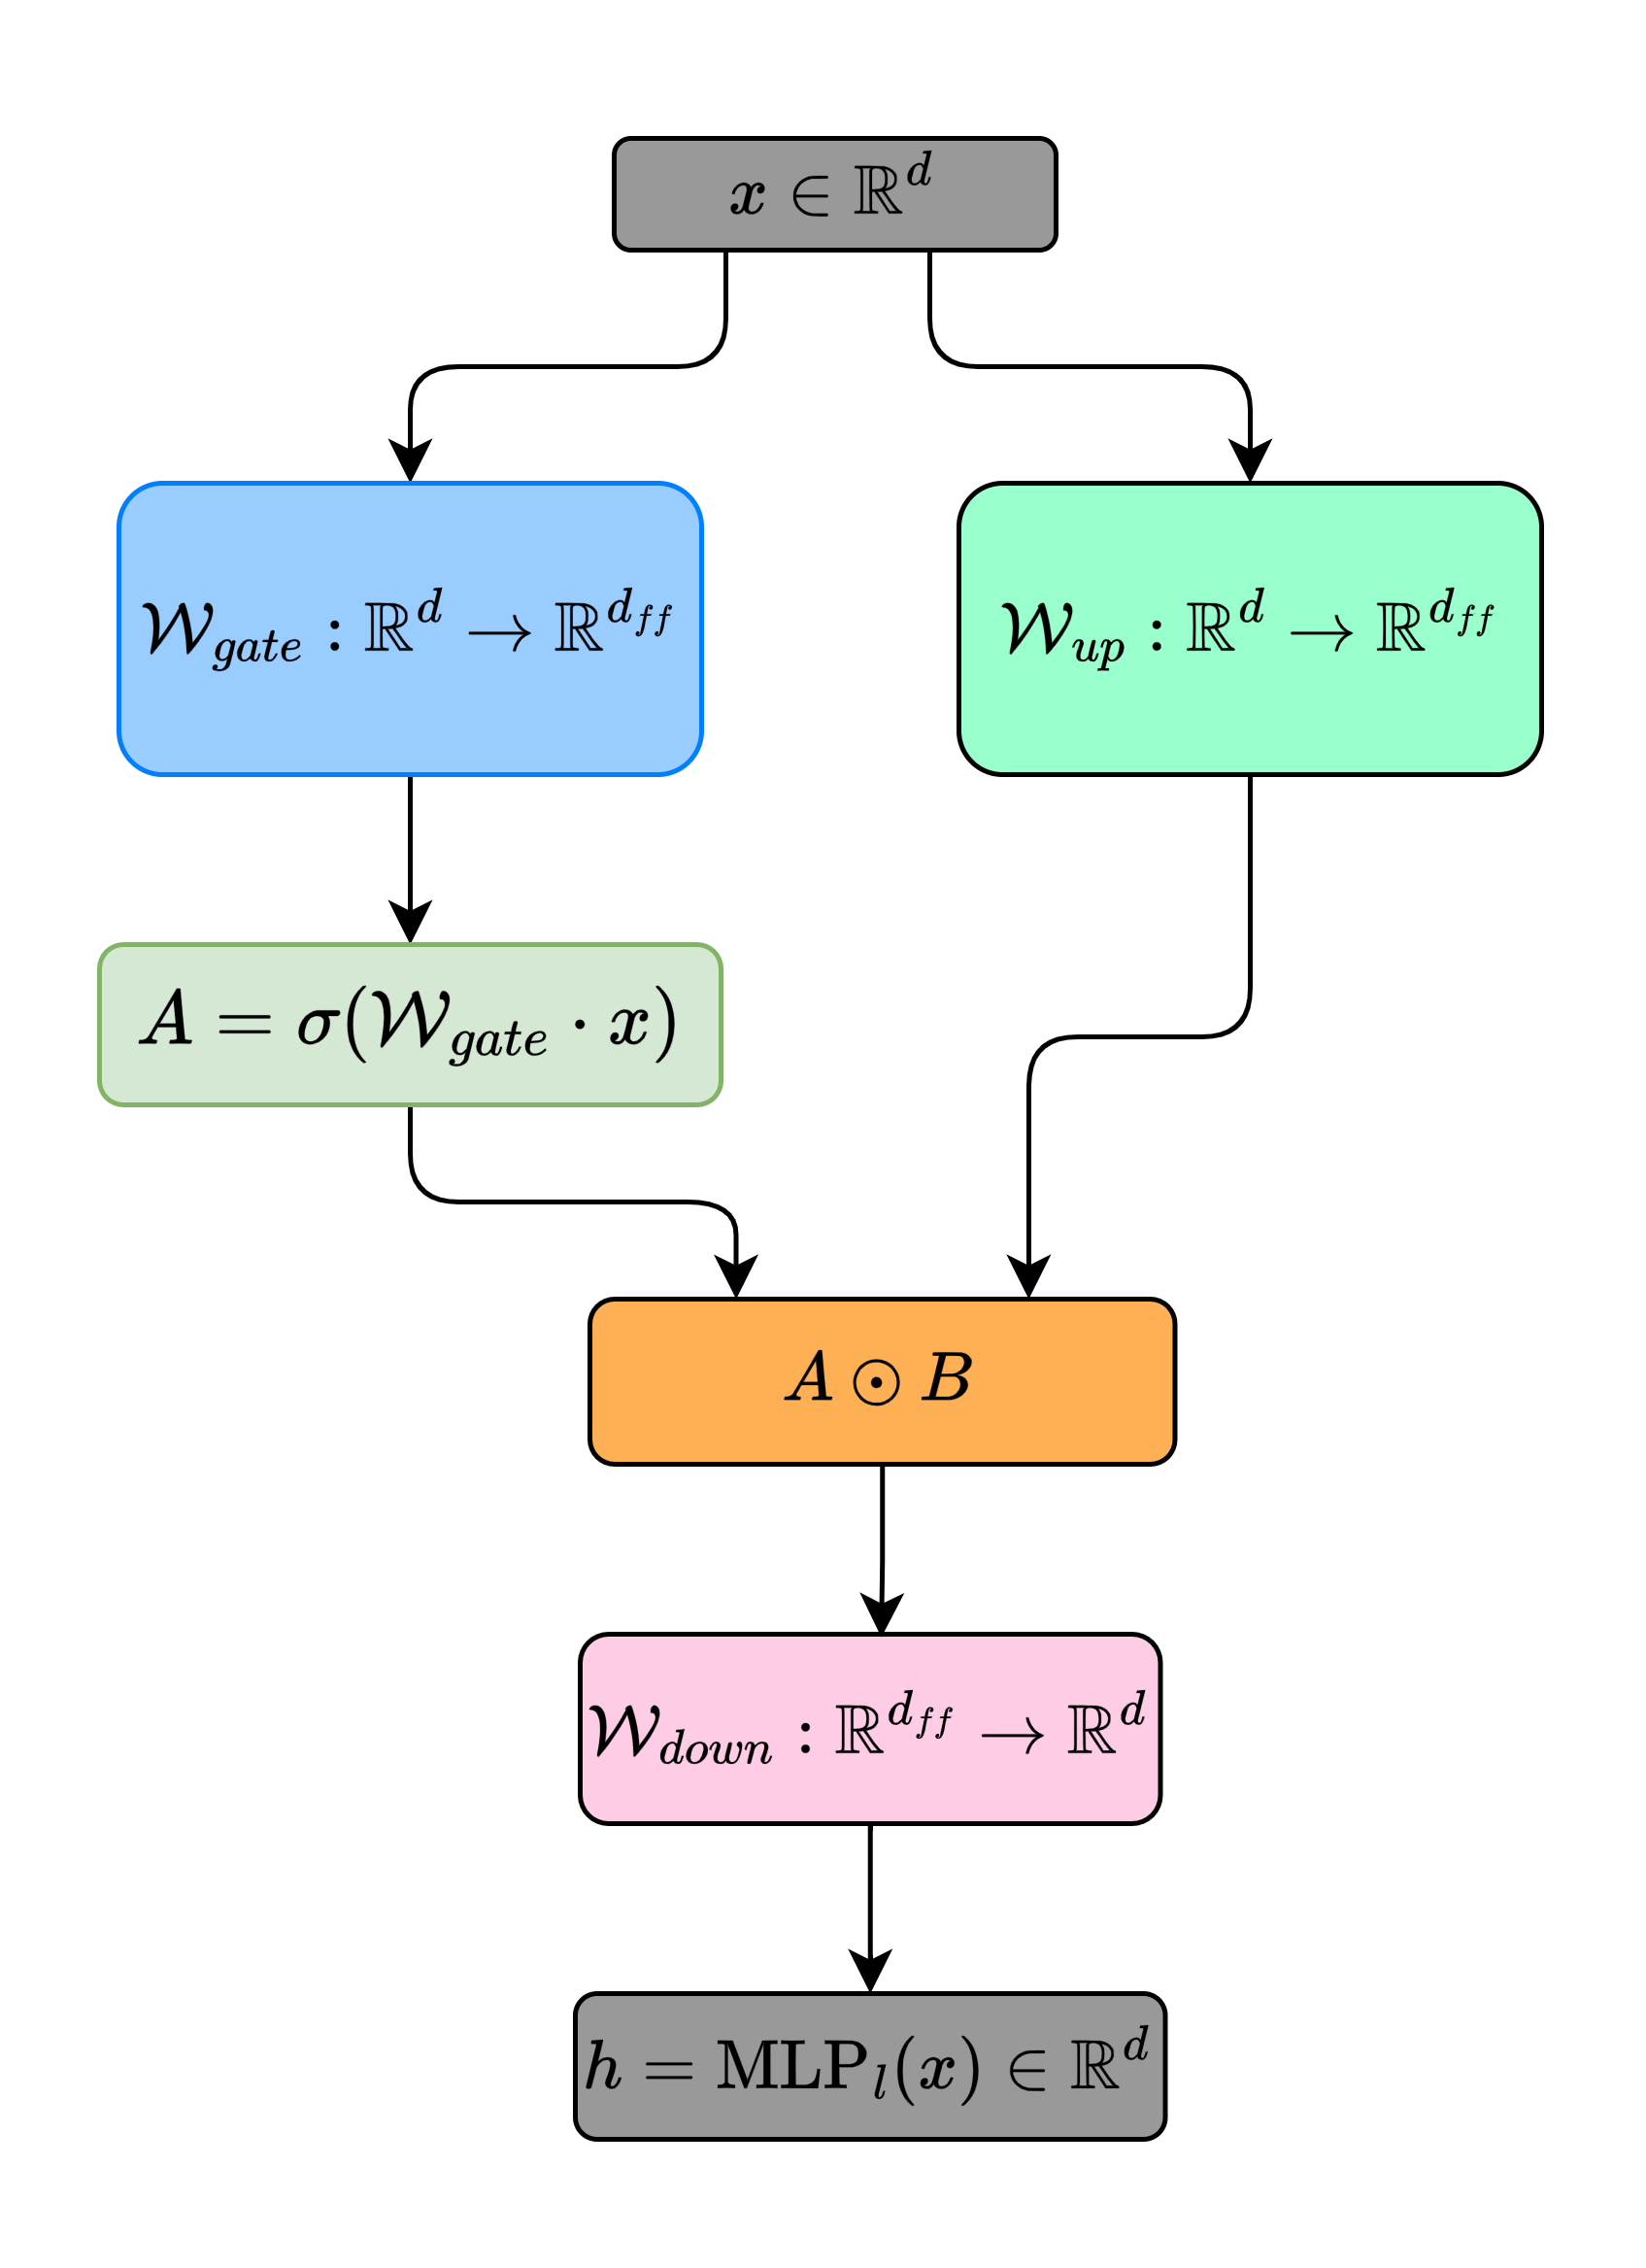
\includegraphics[width=0.35\linewidth]{Images/RePAIR/mlp_architecture.png}
    \caption{SwiGLU MLP in Llama-3-8B: STAMP updates only $W_{\text{down}}$, freezing $W_{\text{gate}}$ and $W_{\text{up}}$.}
    \label{fig:mlp_architecture}
\end{figure}

\medskip
\noindent
\textbf{Steering Vector Computation.} Given the forget pair $(p_f, r_f)$ extracted by $\mathcal{M}_{\textit{watchdog}}$, we construct the forget set $\mathcal{D}_f = \{(p_f, r_f)\}$, the retain buffer $\mathcal{D}_r$ as defined in Section~\ref{subsec:repair_ps}, and a reference set $\mathcal{D}_{\textit{ref}}$ of natural refusal prompts. Notably, $\mathcal{D}_f$ can be a single sample, where most existing methods fail, whereas STAMP operates effectively at this granularity.

We extract MLP activations at layer $l$ for all three sets. Since base models such as Llama-3-8B~\citeauthor{grattafiori2024llama} lack refusal training, we exploit their tendency to echo input. Prompting with ``I don't know'' causes the model to reproduce it as part of the standard prompt-response template, letting us collect refusal-subspace activations without any training. The steering vector, encoding the direction from forget to refusal activations, is computed as:

\begin{equation}
\mathbf{r}_{\textit{SV}} = \frac{1}{|\mathcal{D}_{\textit{ref}}|} \sum_{x \in \mathcal{D}_{\textit{ref}}} \text{MLP}_l(x) - \frac{1}{|\mathcal{D}_f|} \sum_{x \in \mathcal{D}_f} \text{MLP}_l(x) \in \mathbb{R}^d
\label{eq:steering_vector}
\end{equation}

\medskip
\noindent
\textbf{Target Construction.} Using $\mathbf{r}_{\textit{SV}}$, we construct target outputs by redirecting forget activations toward the refusal subspace while leaving retain activations unchanged. We collect the post-activation intermediates $\mathbf{H} = [\mathbf{h}_1; \ldots; \mathbf{h}_n] \in \mathbb{R}^{n \times m}$, the actual input to $W_{\text{down}}$, from $\mathcal{D}_f$, the retain buffer $\mathcal{D}_r$, and $\mathcal{D}_{\textit{ref}}$, and compute desired outputs. If $x \in \mathcal{D}_f$, the steering vector is added to shift the activation toward refusal, that is $\mathbf{o}'(x) = \text{MLP}_l(x) + \mathbf{r}_{\textit{SV}}$, otherwise $\mathbf{o}'(x) = \text{MLP}_l(x)$ remains untouched. The final target matrix $O' \in \mathbb{R}^{n \times d}$ is obtained by stacking all $\mathbf{o}'(x)$ across samples.

Given the original MLP output $O = \mathbf{H} \cdot W_{\text{old}}$, with $W_{\text{old}} \in \mathbb{R}^{m \times d}$ written to match this row-wise convention, we seek $W_{\text{new}}$ such that $O' = \mathbf{H} \cdot W_{\text{new}}$:

\begin{equation}
\mathbf{H} \cdot W_{\text{new}} = O' \quad \therefore \quad W_{\text{new}} = \mathbf{H}^{-1} O'
\label{eq:naive_inverse}
\end{equation}

\medskip
\noindent
\textbf{STAMP: Pseudoinverse Solution.} Since $\mathbf{H}$ is generally non-square and, in the single-sample regime IMU demands, severely rank-deficient ($n \ll m$), we employ the Moore-Penrose pseudoinverse, which provides the minimum-norm least-squares solution. We compute $\mathbf{H}^+ = (\mathbf{H}^\top \mathbf{H} + \lambda I)^{-1} \mathbf{H}^\top \in \mathbb{R}^{m \times n}$, where $\lambda$ is a regularization coefficient for numerical stability and $I$ is the identity matrix. This yields the closed-form weight update:

\begin{equation}
W_{\text{new}} = \mathbf{H}^+ \cdot O' = (\mathbf{H}^\top \mathbf{H} + \lambda I)^{-1} \mathbf{H}^\top O' \in \mathbb{R}^{m \times d}
\label{eq:pseudoinverse}
\end{equation}

applied to $W_{\text{down}}$. The computational bottleneck lies in inverting $(\mathbf{H}^\top \mathbf{H} + \lambda I) \in \mathbb{R}^{m \times m}$, which requires $\mathcal{O}(m^3)$ operations, since inverting an $m \times m$ matrix involves solving $m$ linear systems, each costing $\mathcal{O}(m^2)$; materializing the Gram matrix alone occupies $\mathcal{O}(m^2)$ memory, roughly 822 MB in single precision for Llama-3-8B. Both costs are governed by the FFN width $m$ and are paid in full even when forgetting a single sample, motivating a more efficient variant.

\medskip
\noindent
\textbf{STAMP-LR: Low-Rank Solution.} Inspired by parameter-efficient fine-tuning methods such as LoRA~\citeauthor{hu2022lora} we decompose $\mathbf{H}$ into low-rank factors $\mathbf{H} \approx A \cdot B$, where $A \in \mathbb{R}^{n \times r}$, $B \in \mathbb{R}^{r \times m}$, and $r \ll m$, reducing the inversion from an $m \times m$ problem to two $r \times r$ problems. Since $A$ and $B$ are non-square, we compute their pseudoinverses:

\begin{equation}
A^+ = (A^\top A)^{-1} A^\top \in \mathbb{R}^{r \times n}
\label{eq:a_pseudo}
\end{equation}

\begin{equation}
B^+ = B^\top (BB^\top)^{-1} \in \mathbb{R}^{m \times r}
\label{eq:b_pseudo}
\end{equation}

where both $(A^\top A)^{-1}$ and $(BB^\top)^{-1}$ are $r \times r$ inversions. Unlike STAMP, the low-rank decomposition inherently regularizes the solution by constraining it to a rank-$r$ subspace, eliminating the need for explicit regularization $\lambda I$. The final weight update:

\begin{equation}
W_{\text{new}} = B^+ \cdot A^+ \cdot O' \in \mathbb{R}^{m \times d}
\label{eq:lr_update}
\end{equation}

is applied to $W_{\text{down}}$, yielding the complete STAMP-LR update:

\begin{equation}
W_{\text{new}} = B^\top (BB^\top)^{-1} \cdot (A^\top A)^{-1} A^\top \cdot O'
\label{eq:lr_expanded}
\end{equation}

In STAMP, the bottleneck is inverting $(\mathbf{H}^\top \mathbf{H} + \lambda I) \in \mathbb{R}^{m \times m}$ at $\mathcal{O}(m^3)$. STAMP-LR replaces this with two $r \times r$ inversions, $(A^\top A)^{-1}$ and $(BB^\top)^{-1}$, each costing $\mathcal{O}(r^3)$. The remaining matrix multiplications, namely $A^\top A$ at $\mathcal{O}(n \cdot r^2)$, $A^+ \cdot O'$ at $\mathcal{O}(r \cdot n \cdot d)$, and $B^+ \cdot (A^+ O')$ at $\mathcal{O}(r^2 \cdot m)$, are all dominated by $\mathcal{O}(r^2 \cdot m)$ since $r \ll m$, yielding a total solve cost of $\mathcal{O}(r^3 + r^2 \cdot m)$. STAMP-LR also stores only the low-rank factors $A \in \mathbb{R}^{n \times r}$ and $B \in \mathbb{R}^{r \times m}$, that is $\mathcal{O}(r(n+m))$ memory, under 4 MB at $r = 64$ against the roughly 822 MB Gram matrix STAMP must materialize, a reduction of over 200$\times$. This memory gap, more than the asymptotic time alone, is what makes on-device unlearning practical.

\begin{table}[!htbp]
\centering
\caption{Memory and computational cost comparison across methods for a single-layer intervention.}
\label{tab:cost_comparison}
\small
\renewcommand{\arraystretch}{1.3}
\setlength{\tabcolsep}{6pt}
\begin{tabular}{lccc}
\toprule
\textbf{Method} & \textbf{Time Complexity} & \textbf{Memory} & \textbf{Training-Free} \\
\midrule
Full FT & $\mathcal{O}(E \cdot n \cdot L \cdot d \cdot m)$ & ${\sim}6\times$ model & No \\
\rowcolor{gray!15}
LoRA (all $L$) & $\mathcal{O}(E \cdot n \cdot L \cdot r \cdot d)$ & Model + $2rLd$ & No \\
LoRA (1 layer) & $\mathcal{O}(E \cdot n \cdot r \cdot d)$ & Model + $2rd$ & No \\
\rowcolor{gray!15}
STAMP & $\mathcal{O}(n \cdot d \cdot m + m^3)$ & $m^2$ & Yes \\
STAMP-LR & $\mathcal{O}(n \cdot d \cdot m + r^3 + r^2 \cdot m)$ & $r(n+m)$ & Yes \\
\bottomrule
\end{tabular}
\end{table}

%% ------------------------------------------------------------
\subsection{Memory and Computational Analysis}\label{subsec:rp_compute}
%% ------------------------------------------------------------

A forward pass through one MLP layer costs $\mathcal{O}(d \cdot m)$, and a backward pass costs ${\sim}2\times$ forward. Full fine-tuning over $n$ samples for $E$ epochs across $L$ layers thus requires $\mathcal{O}(E \cdot n \cdot L \cdot d \cdot m)$ compute and ${\sim}6\times$ model size in memory, covering weights, gradients, optimizer states, and activations. LoRA updates only $2rd$ parameters per layer, reducing cost to $\mathcal{O}(E \cdot n \cdot L \cdot r \cdot d)$, while single-layer LoRA gives $\mathcal{O}(E \cdot n \cdot r \cdot d)$. All of these scale with $E \cdot n$ and require backpropagation. Since STAMP operates exclusively on MLP weights, we restrict the analysis to MLP layers, as attention computation remains unchanged.

STAMP eliminates this dependence entirely, but not the cost of collecting activations: both variants require a single forward pass to collect $\mathbf{H}$ and $O'$ at $\mathcal{O}(n \cdot d \cdot m)$, with no gradient computation or optimizer states. STAMP additionally inverts $(\mathbf{H}^\top \mathbf{H} + \lambda I) \in \mathbb{R}^{m \times m}$ at $\mathcal{O}(m^3)$, storing $m^2$ entries. STAMP-LR replaces this inversion with two $r \times r$ inversions at $\mathcal{O}(r^3 + r^2 \cdot m)$, storing only the low-rank factors at $\mathcal{O}(r(n+m))$ entries, under 4 MB at $r=64$ against the roughly 822 MB Gram matrix STAMP must materialize for Llama-3-8B, a reduction of over $200\times$. Table~\ref{tab:cost_comparison} summarizes the comparison, and STAMP-LR is the only method combining training-free operation, single-sample capability, and sub-cubic solve complexity.

%% ------------------------------------------------------------
\subsection{Implementation Details}\label{subsec:rp_implementation}
%% ------------------------------------------------------------

All reported STAMP and STAMP-LR results intervene at layer~6 of Llama-3-8B, with regularization coefficient $\lambda = 10^{-4}$ and default rank $r = 64$ for STAMP-LR. Listing~\ref{lst:stamp_code} sketches the three core routines: the steering vector of Equation~\ref{eq:steering_vector}, the STAMP pseudoinverse solve of Equations~\ref{eq:naive_inverse}--\ref{eq:pseudoinverse}, and the STAMP-LR sketched solve of Equations~\ref{eq:a_pseudo}--\ref{eq:lr_update}. The snippets are illustrative, with model loading, activation hooks, and evaluation omitted.

\begin{codebox}
def steering_vector(model, D_ref, D_f):
    # mean MLP output over the refusal prompts
    mu_ref = mlp_outputs(model, D_ref).mean(0)
    # mean MLP output over the forget samples
    mu_f = mlp_outputs(model, D_f).mean(0)
    # direction from forget to refusal (Eq. 2)
    return mu_ref - mu_f


def stamp(model, D_f, D_r, D_ref, lam=1e-4):
    # steering vector at the target layer
    r_sv = steering_vector(model, D_ref, D_f)
    # stack intermediates H (n x m) and MLP outputs O (n x d)
    H, O = collect_activations(model, D_f + D_r + D_ref, layer=6)
    # redirect the forget rows toward the refusal subspace
    O[rows_of(D_f)] += r_sv
    # regularized pseudoinverse solve (Eqs. 6-7), O(m^3)
    W_new = inv(H.T @ H + lam * eye(m)) @ H.T @ O
    # overwrite the down-projection of layer 6
    set_down_proj(model, W_new)


def stamp_lr(model, D_f, D_r, D_ref, r=64):
    # steering vector and activations, as in STAMP
    r_sv = steering_vector(model, D_ref, D_f)
    H, O = collect_activations(model, D_f + D_r + D_ref, layer=6)
    O[rows_of(D_f)] += r_sv
    # sketch H ~ A B with a random row-orthonormal B
    B = qr(randn(r, m))
    A = H @ B.T
    # pseudoinverses of the two small factors (Eq. 8)
    A_plus = inv(A.T @ A) @ A.T
    B_plus = B.T @ inv(B @ B.T)
    # low-rank update (Eq. 9), O(r^3 + r^2 m)
    W_new = B_plus @ (A_plus @ O)
    set_down_proj(model, W_new)
\end{codebox}
\captionof{listing}{Code snippets for STAMP and STAMP-LR. Comments reference the corresponding equations, and helper routines for activation collection and weight replacement are omitted.}
\label{lst:stamp_code}

Together, BackFlush and RePAIR address the two proposed applications from complementary angles, one sanitizing third-party models against hidden backdoors while preserving watermarks, and the other giving end users direct, training-free control over what a deployed model retains. The following chapter reports the experimental validation of both frameworks.